\documentclass[12pt,a4paper]{article}
% Biên dịch: XeLaTeX/Tectonic hoặc pdfLaTeX (vntex).
% TeX Gyre là phông mở đi kèm các bản phân phối TeX thông dụng.
\usepackage{iftex}
\ifPDFTeX
  \usepackage[utf8]{vntex}
  \usepackage{mathptmx}
  \usepackage[scaled=0.92]{helvet}
  \usepackage{courier}
\else
  \usepackage{fontspec}
  \setmainfont{texgyretermes-regular.otf}[
    BoldFont=texgyretermes-bold.otf,ItalicFont=texgyretermes-italic.otf,
    BoldItalicFont=texgyretermes-bolditalic.otf,Ligatures=TeX]
  \setsansfont{texgyreheros-regular.otf}[
    BoldFont=texgyreheros-bold.otf,ItalicFont=texgyreheros-italic.otf,
    BoldItalicFont=texgyreheros-bolditalic.otf,Scale=0.9]
  \setmonofont{texgyrecursor-regular.otf}[
    BoldFont=texgyrecursor-bold.otf,ItalicFont=texgyrecursor-italic.otf,
    BoldItalicFont=texgyrecursor-bolditalic.otf,Scale=0.88]
\fi
\usepackage{amsmath,amssymb}
\ifPDFTeX\else
  \usepackage{unicode-math}
  \setmathfont{texgyretermes-math.otf}
\fi
\usepackage{geometry,graphicx,titlesec}
\usepackage[table]{xcolor}
\usepackage{caption,float,enumitem,tabularx,array,booktabs,indentfirst}
\usepackage{fancyvrb,fancyhdr,microtype}
\geometry{a4paper,left=2.3cm,right=2.3cm,top=2.4cm,bottom=2.3cm,
  headheight=14pt,headsep=16pt,footskip=25pt}
\definecolor{ink}{HTML}{20252B}
\definecolor{darkblue}{HTML}{18384D}
\definecolor{muted}{HTML}{606A73}
\definecolor{lightblue}{HTML}{F2F5F7}
\definecolor{rulegray}{HTML}{CDD3D8}
\color{ink}
\titleformat{\section}{\normalfont\fontsize{14}{17}\selectfont\bfseries}{\thesection}{0.65em}{}
\titleformat{\subsection}{\normalfont\normalsize\bfseries}{\thesubsection}{0.65em}{}
\titlespacing*{\section}{0pt}{14pt}{7pt}
\titlespacing*{\subsection}{0pt}{10pt}{5pt}
\setlength{\fboxsep}{8pt}
\setlength{\fboxrule}{0.4pt}
\newcommand{\infobox}[2][]{\par\smallskip\noindent
  \fcolorbox{rulegray}{lightblue}{\parbox{\dimexpr\linewidth-2\fboxsep-2\fboxrule\relax}{
  \small\textbf{#1}\par\smallskip #2}}\par\smallskip}
\usepackage[unicode,pdfversion=1.7,colorlinks=true,linkcolor=darkblue,urlcolor=darkblue,citecolor=darkblue]{hyperref}
\hypersetup{pdftitle={Thiet ke va danh gia cac tien ich user-space tren xv6-riscv},
  pdfauthor={Phan Lê Đăng Khoa; Âu Bảo Trân; Dương Nhựt Duy},
  pdfsubject={Bao cao thuc hanh He dieu hanh -- Lab 01},bookmarksnumbered=true}
\setlength{\parindent}{1.25em}
\setlength{\parskip}{3pt}
\linespread{1.1}
\emergencystretch=1em
\setlist{leftmargin=1.6em,itemsep=2pt,topsep=4pt,parsep=0pt}
\setcounter{tocdepth}{2}
\renewcommand{\contentsname}{Mục lục}
\renewcommand{\figurename}{Hình}
\renewcommand{\tablename}{Bảng}
\renewcommand{\refname}{Tài liệu tham khảo}
\newcolumntype{Y}{>{\raggedright\arraybackslash}X}
\newcolumntype{P}[1]{>{\raggedright\arraybackslash}p{#1}}
\renewcommand{\arraystretch}{1.2}
\setlength{\tabcolsep}{6pt}
\captionsetup{font=small,labelfont=bf,labelsep=period,
  justification=raggedright,singlelinecheck=false,skip=7pt}
\captionsetup[table]{position=top}
\newcommand{\code}[1]{\texttt{#1}}
\DefineVerbatimEnvironment{terminal}{Verbatim}{fontsize=\small,frame=leftline,
  rulecolor=\color{rulegray},framerule=1pt,framesep=9pt,baselinestretch=1.05}
\pagestyle{fancy}
\fancyhf{}
\fancyhead[L]{\sffamily\fontsize{8}{10}\selectfont\color{muted}HỆ ĐIỀU HÀNH\enspace /\enspace LAB 01}
\fancyhead[R]{\sffamily\fontsize{8}{10}\selectfont\color{muted}xv6-riscv}
\fancyfoot[C]{\small\thepage}
\renewcommand{\headrulewidth}{0.3pt}
\renewcommand{\footrulewidth}{0pt}
\fancypagestyle{plain}{\fancyhf{}\fancyfoot[C]{\small\thepage}\renewcommand{\headrulewidth}{0pt}}

\begin{document}
\hypersetup{pageanchor=false}
\begin{titlepage}
\thispagestyle{empty}
\centering
\begin{center}
{\small\bfseries TRƯỜNG ĐẠI HỌC KHOA HỌC TỰ NHIÊN, ĐHQG-HCM}\\[4pt]
{\small KHOA CÔNG NGHỆ THÔNG TIN}
\end{center}
\vspace{0cm}
\begin{center}
\includegraphics[width=4cm]{Logo_Truong.png}\end{center}
\vspace*{0.4cm}
{\sffamily\small\bfseries\color{muted}BÁO CÁO THỰC HÀNH HỆ ĐIỀU HÀNH}\\[0.5cm]
{\fontsize{30}{35}\selectfont\bfseries\color{darkblue}Lab 01}\\[0.35cm]
{\fontsize{23}{29}\selectfont\bfseries Thiết kế và đánh giá các tiện ích\\trên xv6-riscv}\\[0.4cm]
{\large\color{muted}Xv6 User Programs: File System}
\par\vspace{0.65cm}
{\color{darkblue}\rule{0.8\textwidth}{0.7pt}}
\par\vspace{0.65cm}
\begin{tabularx}{0.8\textwidth}{@{}p{0.28\textwidth}Y@{}}
\textbf{Lớp} & \textbf{Giảng viên hướng dẫn}\\[3pt]
CQ2024/22 & ThS. Lê Viết Long\\
 & ThS. Phạm Tuấn Sơn\\
\end{tabularx}
\par\vspace{0.65cm}
\textbf{Nhóm thực hiện}\par\smallskip
\begin{tabularx}{0.8\textwidth}{@{}>{\centering\arraybackslash}X>{\centering\arraybackslash}p{3.3cm}@{}}
\toprule
\rowcolor{lightblue}
\textbf{Họ và tên} & \textbf{Mã số sinh viên}\\
\midrule
Phan Lê Đăng Khoa & 24120347\\
Âu Bảo Trân & 24120468\\
Dương Nhựt Duy & 24120293\\
\bottomrule
\end{tabularx}\par
\vfill
{\small\color{muted}Thủ Đức, TP. Hồ Chí Minh}\par
\end{titlepage}
\pagenumbering{roman}
\hypersetup{pageanchor=true}
\thispagestyle{plain}
\tableofcontents
\clearpage
\pagenumbering{arabic}

% =================== NỘI DUNG: TRANG 1 ===================
\begin{center}
{\large\bfseries Thiết kế và đánh giá các tiện ích trên xv6-riscv}\par
\vspace{4pt}
{\small Phan Lê Đăng Khoa\quad Âu Bảo Trân\quad Dương Nhựt Duy}
\end{center}
\vspace{3pt}
\begingroup\small
\noindent\textbf{Tóm tắt.} Báo cáo trình bày thiết kế và kiểm chứng bảy tiện ích trong không gian người dùng trên xv6-riscv. Nhóm tiện ích quản lý tiến trình thực hiện chờ theo nhịp đồng hồ, trao đổi dữ liệu hai chiều và sàng số nguyên tố bằng chuỗi tiến trình nối qua pipe. Nhóm tiện ích thao tác với hệ thống tệp thực hiện sao chép, so sánh theo dòng, duyệt cây thư mục và tổng hợp kích thước tệp. Thực nghiệm trên QEMU sử dụng các kiểm thử MIT phù hợp với đề bài và các chương trình hỗ trợ chạy trực tiếp trong xv6. Kết quả đạt 5/5 kiểm thử MIT, 50/50 điểm bộ tiến trình mở rộng và 70/70 điểm bộ tích hợp; riêng năm nhóm kiểm thử chức năng và xử lý lỗi gồm 86 ca. Báo cáo phân tích cơ chế kết thúc, quản lý tài nguyên và giới hạn của từng giải pháp. Các điểm trên thuộc thang đánh giá nội bộ, không quy đổi thành điểm môn học.
\par\smallskip
\noindent\textbf{Từ khóa:} xv6-riscv; lời gọi hệ thống; pipe; hệ thống tệp; kiểm thử tự động.
\endgroup
\vspace{5pt}
\section{Giới thiệu}\label{sec:intro}
\subsection{Tổng quan và mục tiêu}
Lab 01 tìm hiểu cách xây dựng chương trình trong không gian người dùng trên xv6-riscv thông qua bảy tiện ích: \code{sleep}, \code{pingpong}, \code{primes}, \code{cp}, \code{tree}, \code{du} và \code{diff}. Phạm vi chức năng được xác định theo đề \code{CQ\_Lab01.docx}; tài liệu MIT cung cấp cơ sở đối chiếu cho ba tiện ích về tiến trình~\cite{assignment,mit-util}.

Hai nhóm vấn đề chính gồm quản lý tiến trình và giao tiếp qua pipe (ống dẫn dữ liệu), cùng với thao tác trên hệ thống tệp. Mục tiêu là giải thích luồng dữ liệu, điều kiện kết thúc tệp (EOF) và cách quản lý bộ mô tả tệp (file descriptor, FD), đồng thời kiểm chứng kết quả bằng kiểm thử tự động. Tiêu chí đánh giá gồm tính đúng của đầu ra, mã thoát và khả năng xử lý lỗi tài nguyên.

\subsection{Câu hỏi đánh giá và tiêu chí kiểm chứng}
Nội dung thực nghiệm tập trung vào ba câu hỏi:
\begin{enumerate}[label=\textbf{RQ\arabic*.},leftmargin=2.8em]
\item Các tiến trình có thể trao đổi dữ liệu và kết thúc đúng thứ tự bằng pipe mà vẫn quản lý được FD và tiến trình con hay không?
\item Các phép sao chép, so sánh và tổng hợp kích thước có đáp ứng quy ước đã xác định khi gặp EOF, tệp rỗng, dữ liệu nhị phân hoặc dòng dài hay không?
\item Chương trình phản hồi như thế nào trước đối số sai, đường dẫn vượt giới hạn và tình huống thiếu tài nguyên?
\end{enumerate}
Tính đúng được đánh giá bằng cách đối chiếu đầu ra và mã thoát với giá trị kỳ vọng, đồng thời kiểm tra chương trình hoàn tất trong thời gian cho phép. Thực nghiệm tập trung vào kiểm chứng chức năng, không đo lường hiệu năng.

\subsection{Tổ chức báo cáo}
Mục~\ref{sec:design} mô tả thuật toán và quy tắc quản lý tài nguyên. Mục~\ref{sec:testing} trình bày phương pháp, ma trận kiểm thử và bằng chứng thực nghiệm. Mục~\ref{sec:limits} phân tích khó khăn, giới hạn và các điều kiện chưa được kiểm chứng.

\clearpage
% =================== NỘI DUNG: TRANG 2 ===================
\subsection{Môi trường triển khai và cấu hình máy}
Bảng~\ref{tab:env} trình bày môi trường quan sát khi kiểm thử ngày 15/10/2026. Dung lượng RAM trong bảng là tài nguyên được WSL2 cấp cho Linux. Cấu hình công cụ được ghi nhận để tái lập thí nghiệm theo hướng dẫn môi trường xv6~\cite{mit-tools}.
\begin{table}[H]
\centering\small
\caption{Môi trường thực nghiệm; cấu hình máy giả lập lấy từ Makefile và kernel.}
\label{tab:env}
\begin{tabularx}{\textwidth}{@{}P{3.5cm}Y@{}}
\toprule
\rowcolor{lightblue}
\textbf{Thành phần} & \textbf{Cấu hình đã xác minh}\\
\midrule
Hệ điều hành chủ & Ubuntu 24.04.5 LTS trên WSL2; kernel Linux 6.6.87.2; kiến trúc x86\_64.\\
CPU và bộ nhớ khả dụng & AMD Ryzen 5 5600H; 6 nhân/12 luồng được WSL2 nhận diện; khoảng 15 GiB RAM được cấp cho Linux.\\
Công cụ & RISC-V GCC 13.3.0; QEMU 8.2.2; Python 3.12.3; GNU Make.\\
Máy giả lập xv6 & RISC-V \code{virt}, 128 MiB RAM, 3 CPU ảo; đĩa \code{fs.img} qua virtio-blk.\\
Bản mã nguồn & Nhánh \code{util}, commit \code{35ba531}; bản gốc \code{79e8024}.\\
Giới hạn kernel & \code{NPROC=64}, \code{NOFILE=16}, \code{MAXPATH=128}; tên mục thư mục tối đa \code{DIRSIZ=14} byte.\\
\bottomrule
\end{tabularx}
\end{table}

\subsection{Kiến trúc chương trình và giao diện lời gọi hệ thống}
Shell thực thi các tiện ích thông qua \code{fork}/\code{exec}; phần xử lý nằm trong không gian người dùng. Nhóm tiến trình sử dụng \code{pipe}, \code{read}, \code{write}, \code{wait} và đồng hồ kernel. Nhóm thao tác tệp sử dụng \code{open}, \code{fstat}, \code{read}, \code{write} và \code{close}. Thư viện người dùng cung cấp các hàm xử lý chuỗi, cấp phát bộ nhớ và định dạng; lời gọi hệ thống chuyển yêu cầu đến kernel. Cách phân lớp này cho phép bổ sung tiện ích trên giao diện kernel có sẵn.

\subsection{Tích hợp và quy trình biên dịch}
Bảy chương trình có tệp C tương ứng trong \code{user/} và được thêm vào \code{UPROGS}. Makefile liên kết chúng với thư viện người dùng của xv6, sau đó \code{mkfs} đóng gói vào \code{fs.img}; \code{make qemu} khởi động kernel và shell. Phần triển khai giữ nguyên kernel và bộ kiểm thử MIT.

Bản kiểm thử được xuất từ commit \code{35ba531} sang thư mục tạm bằng \code{git archive HEAD}. Tại bản sao này, nhóm chạy ba bước:
\begin{terminal}
make clean
make -j4 kernel/kernel fs.img
make check-lab01
\end{terminal}
Thư mục riêng giúp cô lập dữ liệu và các tệp sinh ra khi kiểm thử. Mã C được biên dịch với \code{-Wall -Werror}; nhật ký và định danh commit được lưu cùng kết quả để truy vết~\cite{evidence}.

\clearpage
% =================== NỘI DUNG: TRANG 3 ===================
\section{Thiết kế và triển khai}\label{sec:design}
\subsection{\texttt{sleep}: chờ theo nhịp đồng hồ kernel}
\textbf{Mục tiêu.} \code{sleep ticks} tạm dừng tiến trình theo số nhịp đồng hồ (tick) của kernel. Giá trị đầu vào được hiểu theo đơn vị tick, không quy đổi trực tiếp thành giây.

\textbf{Cách tiếp cận.} Chương trình nhận đúng một đối số. Trước khi gọi \code{atoi}, chương trình kiểm tra chuỗi không rỗng, chỉ gồm chữ số và biểu diễn giá trị trong miền $0\ldots 2147483647$. Kiểm tra trước phép nhân và cộng giúp tránh tràn số khi phân tích đối số. Với dữ liệu hợp lệ, chương trình gọi \code{sleep(ticks)} và kết thúc bằng \code{exit(0)}.

\textbf{Trường hợp biên.} Đối số bị thiếu hoặc dư, số âm, ký tự không hợp lệ và giá trị vượt miền biểu diễn đều được báo qua \code{stderr}, kèm mã thoát 1. \code{sleep 0} là hợp lệ. Với \code{sleep 10}, khoảng thời gian đo bằng \code{uptime()} phải đạt ít nhất 10 tick; lịch thực thi có thể làm giá trị quan sát lớn hơn yêu cầu.

\subsection{\texttt{pingpong}: trao đổi một byte hai chiều}
\textbf{Mục tiêu.} Tiến trình cha gửi một byte cho con. Tiến trình con in mã định danh tiến trình (PID) cùng \code{received ping}, rồi gửi lại một byte; cha nhận phản hồi và in PID cùng \code{received pong}.

\textbf{Cách tiếp cận.} Hai pipe một chiều được tạo trước \code{fork}: \code{tochild} truyền từ cha đến con, \code{toparent} truyền theo chiều ngược lại. Mỗi bên đóng ngay hai đầu không sử dụng. Con in ping trước khi gửi phản hồi; cha chỉ in pong sau khi đọc thành công. Sự phụ thuộc dữ liệu này bảo đảm thứ tự ping trước pong.
\infobox[Luồng giao tiếp]{
\centering\small
Cha: ghi 1 byte $\xrightarrow{\texttt{tochild}}$ Con: đọc, in ping\\[3pt]
Cha: đọc, in pong $\xleftarrow{\texttt{toparent}}$ Con: ghi trả 1 byte
}
\textbf{Quản lý tài nguyên.} Kết quả mỗi lần \code{read}/\code{write} được kiểm tra để bảo đảm truyền đủ một byte. Sau trao đổi, hai bên đóng các đầu pipe; cha gọi \code{wait} và kiểm tra trạng thái con. Nếu tạo pipe hoặc \code{fork} thất bại, các FD đã mở được đóng. Mã thoát là 0 khi thành công và 1 khi có lỗi.

\subsection{\texttt{primes}: sàng nguyên tố bằng pipeline tiến trình}
\textbf{Mục tiêu và thuật toán.} Tiến trình phát gửi các số nguyên từ 2 đến 280, mỗi số 4 byte. Tầng lọc đọc số đầu làm nguyên tố $p$, in \code{prime p}, loại các bội của $p$ và chuyển phần còn lại sang tầng sau. Số đến đầu tiên của tầng kế tiếp không có ước nguyên tố nhỏ hơn, nên là số nguyên tố tiếp theo.

\textbf{Tạo tầng khi cần.} Chỉ khi tìm thấy số không bị loại, tầng hiện tại mới tạo pipe và gọi \code{fork}. Tiến trình con thay FD đầu vào rồi tiếp tục vòng lặp. Mỗi nguyên tố có một tiến trình riêng; cách triển khai này không làm tăng độ sâu ngăn xếp do lời gọi đệ quy. Kết quả kỳ vọng gồm 59 số, từ 2 đến 277.

\textbf{Kết thúc và tài nguyên.} Mỗi tầng đóng đầu ghi trước khi gọi \code{wait}, cho phép tầng sau nhận EOF sau khi đọc hết dữ liệu còn lại. Chuỗi chờ con truyền trạng thái lỗi về tiến trình phát và bảo đảm tiến trình chính chỉ thoát khi toàn bộ pipeline kết thúc. Phạm vi 2--280 tuân theo đề bài và giới hạn tài nguyên xv6.

\clearpage
% =================== NỘI DUNG: TRANG 4 ===================
\subsection{\texttt{cp}: sao chép nội dung tệp}
\textbf{Mục tiêu.} \code{cp src dst} sao chép tệp thông thường, tạo tệp đích mới hoặc ghi đè nội dung đã tồn tại.

\textbf{Cách tiếp cận.} Chương trình mở nguồn bằng \code{O\_RDONLY} và kiểm tra loại tệp qua \code{fstat}. Nếu đích tồn tại, loại tệp và cặp \code{dev}/\code{ino} được đối chiếu trước khi mở đích bằng \code{O\_WRONLY | O\_CREATE | O\_TRUNC}. Cặp định danh này nhận diện được hai đường dẫn cùng tham chiếu một tệp qua liên kết cứng (hard link), giúp tránh cắt ngắn chính tệp nguồn.

Dữ liệu được đọc theo bộ đệm 1024 byte. Với mỗi khối $n$ byte, chương trình ghi lặp đến khi đủ $n$ byte rồi mới đọc tiếp, thay vì giả định một lần \code{write} luôn hoàn tất yêu cầu. Quá trình sao chép dừng khi gặp EOF; các FD đã mở được đóng trước khi kết thúc.

\textbf{Trường hợp biên và giới hạn.} \code{O\_TRUNC} loại phần đuôi cũ khi ghi đè tệp dài bằng tệp ngắn. Tệp rỗng, dữ liệu nhị phân và tệp lớn hơn bộ đệm được xử lý theo số byte thực tế. Chương trình trả 0 khi thành công; lỗi đối số, loại tệp hoặc thao tác vào/ra có thông báo và mã thoát 1. Lỗi ghi giữa chừng có thể để lại tệp đích chưa đầy đủ; bản triển khai chưa hỗ trợ sao chép nguyên tử hoặc khôi phục nội dung cũ.

\subsection{\texttt{diff}: so sánh hai tệp theo vị trí dòng}
\textbf{Mục tiêu.} \code{diff file1 file2 [-q]} so sánh các dòng cùng vị trí. Hai tệp giống nhau không tạo đầu ra; khác biệt được đánh dấu \code{<} cho tệp thứ nhất và \code{>} cho tệp thứ hai. Tùy chọn \code{-q} có thể đứng trước hoặc sau hai tên tệp.

\textbf{Đọc và so sánh.} Hàm \code{read\_line} đọc đến ký tự xuống dòng hoặc EOF, trả cả độ dài và nội dung. Bộ đệm ban đầu 128 byte được tăng gấp đôi khi cần. So sánh độ dài và từng byte giúp phân biệt ký tự xuống dòng cuối, đồng thời xử lý byte NUL (giá trị 0) bên trong dữ liệu. Hai bộ đệm được tái sử dụng rồi giải phóng khi kết thúc.

\textbf{Quy ước đầu ra.} Chương trình in \code{< tệp:dòng: nội-dung} hoặc \code{> tệp:dòng: nội-dung}. Khi một tệp kết thúc trước, chỉ các dòng còn lại của tệp kia được in, không bổ sung dòng báo EOF. Ví dụ, với \code{f1} chứa một dòng và \code{f2} có thêm dòng \code{two}, kết quả chạy thật là:
\begin{terminal}
$ diff f1 f2
> f2:2: two
\end{terminal}
Vị trí ký hiệu \code{<}/\code{>} và cách biểu diễn EOF khác ví dụ định dạng trong đề~\cite{assignment}. Dòng cuối thiếu ký tự xuống dòng được báo bằng \code{\textbackslash{} No newline at end of file}. Bộ kiểm thử nội bộ đối chiếu các quy ước này; kết quả đạt chưa xác nhận yêu cầu định dạng của bộ chấm giảng viên.

\textbf{Chế độ yên lặng và lỗi.} Với \code{-q}, chương trình dừng tại khác biệt đầu tiên và chỉ in \code{diff: files differ}. Mã thoát là 0 nếu bằng nhau, 1 nếu khác và 2 nếu có lỗi. Lỗi mở, loại tệp, đọc hoặc cấp phát được báo rõ; các FD và bộ nhớ đã cấp phát được thu hồi.

\textbf{Giới hạn thuật toán.} Chương trình ghép dòng theo số thứ tự, không tìm dãy con chung dài nhất để tối ưu phép chèn hoặc xóa. Thời gian xử lý tuyến tính theo lượng dữ liệu đọc; bộ nhớ tỉ lệ với hai dòng dài nhất. Đọc từng byte tạo nhiều lời gọi hệ thống với tệp lớn; độ dài dòng vẫn chịu giới hạn bộ nhớ và ngưỡng cấp phát.

\clearpage
% =================== NỘI DUNG: TRANG 5 ===================
\subsection{\texttt{tree}: duyệt và biểu diễn cây thư mục}
\textbf{Mục tiêu.} \code{tree [path] [-L depth] [-d]} in cấu trúc phân cấp. Đường dẫn mặc định là \code{.}; \code{-L} giới hạn độ sâu, \code{-d} chỉ hiển thị thư mục.

\textbf{Cách tiếp cận.} Mỗi thư mục được mở chỉ đọc, kiểm tra bằng \code{fstat} và duyệt các \code{struct dirent} qua \code{read}. Chương trình bỏ mục không sử dụng, \code{.} và \code{..}, sau đó gọi \code{stat} để lọc loại tệp và quyết định đệ quy. Ký hiệu hiển thị thống nhất là \code{|--} và \code{|\ \ \ }; thứ tự theo các mục trên đĩa, không sắp xếp theo tên.

Độ sâu hiển thị được tính từ gốc là 0, trong khi biến mức của hàm bắt đầu từ 1. Vì vậy, \code{-L 0} chỉ in gốc, \code{-L 1} in thêm các mục con trực tiếp. Tùy chọn \code{-d} chỉ giữ thư mục trong đầu ra. Chương trình nhận tối đa một đường dẫn; tùy chọn có thể đứng trước hoặc sau đường dẫn.

\textbf{An toàn dữ liệu và lỗi.} Trường \code{dirent.name} có 14 byte và có thể thiếu NUL kết thúc. Tên được chép sang bộ đệm 15 byte rồi thêm NUL trước khi xử lý bằng hàm chuỗi. Đường dẫn gốc và đường dẫn ghép dài tối đa 127 byte, chừa một byte NUL trong \code{MAXPATH=128}. Lỗi mở, đọc, \code{stat} hoặc duyệt nhánh con được truyền về gốc; chương trình trả mã 1 khi có lỗi và đóng FD trước khi rời mỗi tầng.

\subsection{\texttt{du}: tổng hợp kích thước theo byte}
\textbf{Mục tiêu và quy ước.} \code{du [path] [-a] [-s]} tính tổng kích thước logic của tệp theo \code{st.size}, đơn vị byte. Phép tính không cộng kích thước bản thân thư mục và không đo số khối đĩa cấp phát. Thư mục rỗng và thiết bị được tính 0 byte. Quy ước bỏ kích thước bản thân thư mục được đề cho phép nếu trình bày nhất quán~\cite{assignment}.

Với thư mục $d$, giá trị được tính hậu thứ tự:
\[
 S(d)=\sum_{x\in\mathrm{con}(d)} S(x),\qquad
 S(f)=\mathrm{st.size}(f)\quad\text{với tệp thông thường }f.
\]
\textbf{Cách tiếp cận.} Chương trình duyệt các mục và nối đường dẫn như \code{tree}; tính từng cây con, cộng vào tổng \code{uint64}, sau đó mới in thư mục cha. Trạng thái lỗi được trả riêng với biến tổng để phân biệt lỗi mở với thư mục rỗng. Hàm định dạng thập phân riêng chuyển số 64 bit thành chuỗi, do \code{printf} của bản xv6 này vẫn thu hẹp giá trị qua \code{printint(int)} khi dùng định dạng dài.

\textbf{Quy tắc hiển thị.} Mặc định chỉ in thư mục; \code{-a} in thêm tệp; \code{-s} chỉ in tổng tại gốc và được ưu tiên khi kết hợp với \code{-a}. Nếu gốc là tệp, chỉ \code{-a} hoặc \code{-s} mới tạo đầu ra. Kết quả có dạng \code{bytes\textbackslash{}tpath}. Khi duyệt gặp lỗi, chế độ \code{-s} không xuất tổng chưa đầy đủ và chương trình trả mã thoát 1.

\textbf{Giới hạn chung.} Hai chương trình giữ một FD cho mỗi thư mục tổ tiên; cây sâu có thể chạm giới hạn \code{NOFILE=16}. Khi đó, chương trình báo lỗi và trả trạng thái thất bại. Phép tính của \code{du} cộng theo từng mục thư mục, nên các liên kết cứng đến cùng inode có thể được tính nhiều lần.

\clearpage
% =================== NỘI DUNG: TRANG 6 ===================
\section{Kiểm thử và đánh giá}\label{sec:testing}
\subsection{Phương pháp và khả năng tái lập}
Kiểm thử ngày 15/10/2026 được chạy lại trên bản xuất sạch của commit \code{35ba531}. Lệnh \code{make check-lab01} gọi bộ MIT cho ba tiện ích tiến trình, bộ TV1 mở rộng và bộ tích hợp. Bộ MIT có ca xác minh \code{sys\_sleep}; TV1 lặp \code{pingpong} 50 lần và \code{primes} 20 lần.

Các chương trình hỗ trợ bằng C chạy thật trong xv6 qua QEMU, tạo dữ liệu, thu đầu ra và gọi \code{wait(\&status)} để kiểm tra mã thoát. Từng nhóm tích hợp tạo lại \code{fs.img} để cô lập dữ liệu; các chương trình hỗ trợ chỉ có trong ảnh hệ thống tệp dùng để kiểm thử.

\subsection{Ma trận kiểm thử và kết quả thực tế}
\begin{table}[H]
\centering\small
\caption{Kết quả kiểm thử; 86 ca thuộc năm nhóm chức năng và xử lý lỗi.}
\label{tab:tests}
\renewcommand{\arraystretch}{1.1}
\begin{tabularx}{\textwidth}{@{}P{2.4cm}YP{2.05cm}@{}}
\toprule
\rowcolor{lightblue}
\textbf{Nhóm} & \textbf{Nội dung được đối chiếu tự động} & \textbf{Kết quả}\\
\midrule
Biên dịch & Kernel, hệ thống tệp, bảy tiện ích; \code{-Wall -Werror}. & Đạt\\
MIT & 3 ca \code{sleep}, 1 ca \code{pingpong}, 1 ca \code{primes}. & 5/5 ca\\
TV1 mở rộng & Đối số, tick, mã thoát, kiểm thử lặp và pipeline. & 50/50 điểm\\
\code{cp} & Tệp rỗng, nhị phân 8193 byte, ghi đè, cùng inode; lỗi. & 13/13 ca\\
\code{diff} & EOF, \code{-q}, xuống dòng, NUL, dòng 4098 byte; lỗi. & 23/23 ca\\
\code{tree} & \code{-L 0/1/2}, \code{-d}, tên 14 byte; lỗi đường dẫn và FD. & 21/21 ca\\
\code{du} & Tổng byte, \code{-a/-s}, tệp gốc, rỗng; lỗi đường dẫn và FD. & 17/17 ca\\
Tài nguyên & Cạn FD khi mở tệp, tạo pipe và tạo tầng sàng. & 12/12 ca\\
Định dạng số & Hàm in của \code{du}: $0$, $2^{32}$ và $2^{64}-1$. & 3/3 giá trị\\
Tích hợp & Luồng shell sử dụng đủ bảy tiện ích. & Đạt\\
\bottomrule
\end{tabularx}
\end{table}
\noindent Cả ba bộ kết thúc với mã 0. Hình~\ref{fig:test-summary} trình bày các dòng kết quả được lọc từ nhật ký lần chạy lại; điểm 50/50 và 70/70 thuộc thang nội bộ, không phải điểm môn học~\cite{evidence}.
\begin{figure}[H]
\centering
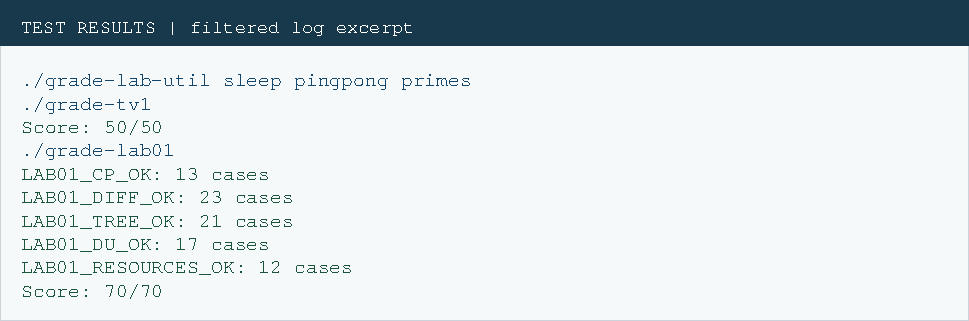
\includegraphics[width=\linewidth]{docs/report-validation/figures/test-summary.pdf}
\caption{Trích đoạn tổng kết kiểm thử, dựng từ nhật ký đã lọc trên commit \code{35ba531}.}
\label{fig:test-summary}
\end{figure}

\clearpage
% =================== NỘI DUNG: TRANG 7 ===================
\subsection{Minh chứng tiêu biểu và phân tích kết quả}
Hình~\ref{fig:workflow} trình bày trích đoạn liên tục từ nhật ký QEMU của luồng tích hợp. Hai tệp cùng chứa \code{hello} và ký tự xuống dòng, mỗi tệp 6 byte; \code{diff -q} không tạo đầu ra và \code{du demo -s} trả tổng 12 byte.
\begin{figure}[H]
\centering
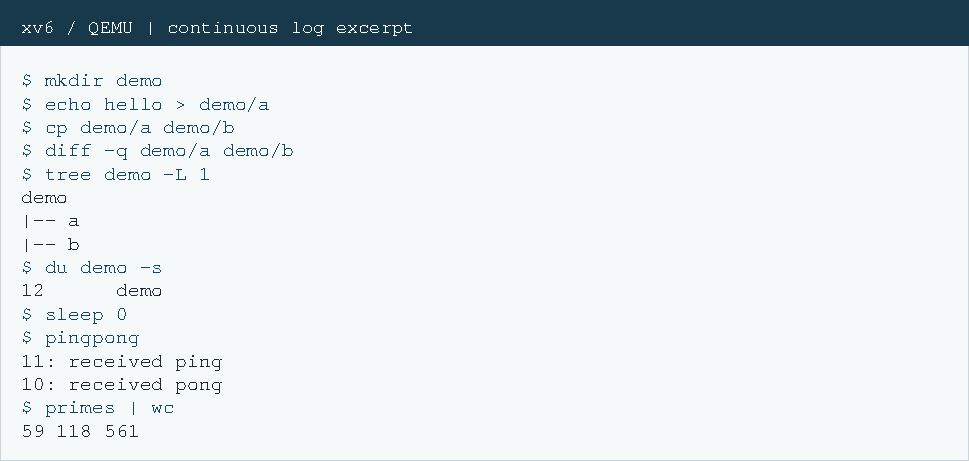
\includegraphics[width=\linewidth]{docs/report-validation/figures/workflow.pdf}
\caption{Luồng tích hợp trong xv6, dựng từ nhật ký QEMU; \code{primes | wc} ghi nhận 59 dòng.}
\label{fig:workflow}
\end{figure}

\textbf{Dữ liệu lớn hơn bộ đệm.} Nội dung nhị phân 8193 byte của \code{cp} được đối chiếu toàn bộ, gồm khối cuối không đầy. Với \code{diff}, dòng 4098 byte có thay đổi sau byte 4096 giúp phát hiện lỗi cắt ngắn; dữ liệu chứa NUL kiểm tra phép so sánh theo độ dài.

\textbf{Định dạng 64 bit.} Hàm in của \code{du} được gọi trực tiếp với $0$, $2^{32}$ và $2^{64}-1$. Kết quả đúng xác minh định dạng số, không chứng minh xv6 đã tạo được tệp có kích thước tương ứng.
\subsection{Thảo luận kết quả và phạm vi hiệu lực}
\textbf{RQ1 -- Tiến trình.} Đầu ra của mỗi lần chạy \code{primes} được đối chiếu với 59 số nguyên tố xác định bằng phép chia thử độc lập. Với \code{pingpong}, 100 thông báo đúng thứ tự có PID khác nhau trong từng cặp. Cả hai trở lại shell và chạy được trong pipeline. Phép đo \code{sleep 10} đạt ít nhất 10 tick.

\textbf{RQ2 -- Dữ liệu.} Các ca tệp rỗng, nhị phân, ghi đè, dòng dài và NUL cho thấy phép xử lý theo byte đáp ứng các trường hợp đã thử. Tổng của \code{du} phù hợp với quy ước kích thước logic.

\textbf{RQ3 -- Lỗi.} Các ca kiểm thử chủ động dùng hết FD để đối chiếu thông báo và mã thoát; giới hạn thời gian giúp phát hiện treo. Duyệt cây 20 cấp thất bại có kiểm soát, còn \code{tree -L 2} thành công khi giới hạn độ sâu.

\textbf{Phạm vi hiệu lực.} Chưa chủ động gây ra mọi lỗi \code{fork}, cạn bộ nhớ, đầy đĩa hoặc thay đổi hệ thống tệp đồng thời. Bộ kiểm thử chưa vét cạn. Thời gian chạy QEMU/WSL2 chịu ảnh hưởng lịch thực thi máy chủ, nên không được dùng để suy luận hiệu năng.

\clearpage
% =================== NỘI DUNG: TRANG 8 ===================
\section{Khó khăn và giới hạn}\label{sec:limits}
\textbf{Thông báo lỗi và mã thoát không nhất quán.} Nhật ký trước tích hợp ghi nhận \code{tree} và \code{du} báo lỗi đường dẫn nhưng vẫn gọi \code{exit(0)}. Nhóm sửa bằng cách truyền trạng thái từ hàm duyệt về \code{main}. Với \code{du}, tách trạng thái lỗi khỏi biến tổng còn giúp chế độ \code{-s} tránh xuất kết quả chưa đầy đủ. Các ca kiểm thử hồi quy cho đường dẫn lỗi đều đạt.

\textbf{Tên mục thư mục có thể thiếu ký tự kết thúc chuỗi.} Tên dài đúng \code{DIRSIZ} có thể thiếu NUL kết thúc; dùng trực tiếp với hàm chuỗi có nguy cơ đọc vượt vùng nhớ. Bản sửa sử dụng bộ đệm \code{DIRSIZ+1}, thêm NUL và kiểm tra độ dài trước khi nối đường dẫn. Các ca tên 14 byte và đường dẫn vượt \code{MAXPATH} kiểm chứng hai điều kiện này.

\textbf{Kiểu dữ liệu và hàm in không đồng nhất.} Tổng của \code{du} dùng \code{uint64}, nhưng đổi định dạng sang \code{\%lu} chưa giải quyết được việc \code{printf} chuyển giá trị vào hàm nhận \code{int}. Hàm chuyển thập phân riêng tránh thu hẹp kiểu. Các ca giá trị lớn ở Mục~\ref{sec:testing} giúp phát hiện hồi quy của lỗi này.

\textbf{EOF và giới hạn tài nguyên.} Giữ đầu ghi pipe không cần thiết có thể khiến tầng sau chờ dữ liệu vô hạn. Vì vậy, đóng FD phải đi cùng thiết kế đồng bộ tiến trình. Với duyệt thư mục, bản triển khai vẫn giữ FD của các thư mục tổ tiên và báo lỗi khi vượt giới hạn. Các ca cạn FD kiểm tra khả năng thất bại có kiểm soát; chúng chưa chứng minh xử lý được mọi tình huống thiếu tài nguyên.

\section{Phân công và đóng góp}
Bảng~\ref{tab:contributions} tổng hợp phần mã nguồn theo hồ sơ bàn giao và trách nhiệm báo cáo theo phân công của nhóm~\cite{source}. Hồ sơ commit xác định phần triển khai; bảng không đánh giá định lượng mức đóng góp cá nhân.
\begin{table}[H]
\centering\small
\caption{Phân công triển khai và tổng hợp báo cáo.}
\label{tab:contributions}
\begin{tabularx}{\textwidth}{@{}P{3.25cm}Y@{}}
\toprule
\rowcolor{lightblue}
\textbf{Thành viên} & \textbf{Phần triển khai và phần báo cáo được giao}\\
\midrule
Phan Lê Đăng Khoa & \code{sleep}, \code{pingpong}, \code{primes}; nhánh \code{lab01-process}, bàn giao \code{a577dd5}. Phân công báo cáo: phần tiến trình, điều phối và rà soát chung.\\
Âu Bảo Trân & \code{cp}, \code{diff}; nhánh \code{lab01-files}, bàn giao \code{bf5cc3a}. Phân công báo cáo: tổng hợp, định dạng, bìa và kết luận.\\
Dương Nhựt Duy & \code{tree}, \code{du}; nhánh \code{lab01-directories}, bàn giao \code{6d9d56a}. Phân công báo cáo: môi trường, kiểm thử và tổng hợp khó khăn.\\
\bottomrule
\end{tabularx}
\end{table}
\noindent\textbf{Khả năng tái lập.} Mã nguồn được xác định bằng commit; các script, chương trình hỗ trợ và nhật ký cho phép đối chiếu từng nhóm kết quả. Minh chứng trong Hình~\ref{fig:test-summary} và Hình~\ref{fig:workflow} được dựng trực tiếp từ nhật ký lần chạy lại, với cách trích xuất lưu cùng bằng chứng~\cite{source,evidence}.
\label{lastcontent}

\clearpage
% =================== PHẦN KẾT: NGOÀI SỐ TRANG NỘI DUNG ===================
\section{Kết luận}
Lab 01 đã triển khai đủ bảy tiện ích trên xv6-riscv và chạy lại thành công các bộ kiểm thử được lựa chọn trong phạm vi bài làm. Kết quả bao phủ các trường hợp thông thường cùng những tình huống biên liên quan đến EOF, dữ liệu lớn hơn bộ đệm, hai đường dẫn cùng trỏ đến một inode, tên tệp dài 14 byte và thiếu FD.

Bài thực hành làm rõ mối liên hệ giữa thuật toán và tài nguyên hệ điều hành. Đóng đúng đầu pipe cho phép bên đọc nhận EOF; chuỗi lời gọi \code{wait} bảo đảm tiến trình phát chỉ thoát sau khi toàn bộ pipeline kết thúc. Thông tin loại tệp và inode hỗ trợ duyệt thư mục và tránh tự ghi đè nguồn. Việc đối chiếu mã thoát cùng dữ liệu kỳ vọng độc lập giúp phát hiện lỗi khó nhận ra qua quan sát đầu ra đơn thuần.

Các giới hạn còn lại gồm phạm vi sàng 2--280, số FD khi duyệt cây sâu, việc tính liên kết cứng theo từng mục thư mục và phép so sánh theo vị trí dòng. Định dạng \code{diff} cần được đối chiếu thêm nếu bộ chấm yêu cầu đầu ra trùng ví dụ của đề. Các hướng phát triển tiếp theo là đọc dòng theo khối, giảm FD giữ khi duyệt cây, bổ sung kiểm thử lỗi cấp phát và ghi đĩa, cũng như cơ chế bảo toàn tệp đích khi sao chép thất bại.

\clearpage
\phantomsection
\addcontentsline{toc}{section}{Tài liệu tham khảo}
\begingroup\small\raggedright
\begin{thebibliography}{9}
\setlength{\itemsep}{7pt}
\bibitem{assignment} Đề bài môn Hệ điều hành, \emph{Lab 01 -- Xv6 User Programs: File System}, tài liệu \code{CQ\_Lab01.docx}. Phạm vi chức năng, tiêu chí đánh giá và quy định nộp bài.
\bibitem{mit-util} MIT, \emph{Lab: Xv6 and Unix utilities}, học phần 6.1810, 2024. Truy cập ngày 15/10/2026.\\
\url{https://pdos.csail.mit.edu/6.1810/2024/labs/util.html}
\bibitem{mit-tools} MIT, \emph{Tools}, học phần 6.1810, 2024. Truy cập ngày 15/10/2026.\\
\url{https://pdos.csail.mit.edu/6.1810/2024/tools.html}
\bibitem{source} Nhóm thực hiện, \emph{Mã nguồn và hồ sơ bàn giao Lab 01}, commit \code{35ba531}; các thư mục \code{user/}, \code{tests/}, \code{docs/lab01/} và \code{docs/tv1/}.\\
\url{https://github.com/EndlessMelody/os-lab1}
\bibitem{evidence} Nhóm thực hiện, \emph{Nhật ký kiểm thử Lab 01 ngày 15/10/2026}, thư mục \code{docs/report-validation/}: môi trường và hồ sơ kiểm chứng; thư mục con \code{upgrade/}: nhật ký biên dịch, kiểm thử, QEMU và ví dụ \code{diff}; thư mục con \code{figures/}: minh chứng cùng nội dung trích xuất. Công cụ dựng hình: \code{tools/render-report-evidence.py}.
\end{thebibliography}
\endgroup
\end{document}
